\documentclass[a4paper,10pt]{scrartcl}
\usepackage[utf8]{inputenc}
\usepackage[hyphens]{url}
\usepackage{hyperref}
\usepackage[ngerman]{babel}
\usepackage[T1]{fontenc}
\usepackage{graphicx}
\usepackage[utf8]{inputenc}
\usepackage{lmodern}
\usepackage{geometry}
\usepackage{pgfplots} 
\usepackage{mathrsfs}
\usepackage{mathtools}
\usepackage{listings}
\usepackage{wrapfig}
\usepackage{float}
\usepackage{amsmath}
\usepackage{stmaryrd}
\usepackage{paralist}
\lstset{basicstyle=\normalfont\ttfamily,breaklines=true}


\geometry{paper=a4paper, left=25mm, right=25mm, top=35mm, bottom=35mm}
\hypersetup{
    unicode=false,
    pdftoolbar=true,
    pdfmenubar=true,
    pdffitwindow=false,
    pdfstartview={FitH},
    pdftitle={DataScienceReport},
    pdfauthor={PaSeDa},
    pdfsubject={Subject},
    pdfcreator={Creator},
    pdfproducer={Producer},
    pdfkeywords={keyword1} {key2} {key3},
    pdfnewwindow=true,
    colorlinks=false,
    linkcolor=red,
    citecolor=green,
    filecolor=magenta,
    urlcolor=cyan
}

\title{\vspace{-2cm}Bericht DataSciece Projekt}
\subtitle{Verbindung von Gehalt und Wahlverhalten in Frankfurt}
\author{PaSeDa}
\date{}

\usepackage{etoolbox}


%Mathepakete
\usepackage{amsfonts}
\usepackage{amsmath}
\usepackage{amssymb}
\usepackage{amsthm}    

\newcommand{\TODO}{\textcolor{red}{\textbf{TODO }}}

\allowdisplaybreaks
\begin{document}
\maketitle

\begin{abstract}Dies ist die finale Ausarbeitung unseres Projektes für das Modul DataScience 1. Untersucht wurde ob ein signifikanter Zusammenhang von Gehalt und Wahlverhalten in Frankfurt besteht. Dazu wurden zwei Datensätze, zu finden auf \lstinline|offendaten.frankfurt.de|, verwendet, die Informationen von Gehalt und Wahlverhalten je Stadtteil zu Verfügung stellen. Organisiert haben war unser Projekt mit Jupyter Notebooks und GitHub. Die gesäuberten Datensätze wurden auf verschiedene Weise untersucht. Insbesondere wurden mehrere Multi-Target-Regressoren trainiert, um festzustellen, ob eine sinnvolle Wahlvorhersage aufgrund des Gehalts möglich ist. Festgestellt haben wir, dass es einen signifikanten Zusammenhang zwischen Verteilung Gehalt eines Stadtteils und den Wählerstimmen für SPD, FDP und AFD gibt.  \end{abstract}

\tableofcontents

\section{Zielsetzung}
Dass das Wahlverhalten von Deutschen durch ihre Einkommen beeinflusst werde, ist etwas, dass viele schon gehört haben oder auch selber vermuten. Wir wollen diese These an Hand von Daten aus Frankfurt untersuchen.

\section{Unsere Infrastruktur}
Unser gesamtes Projekt ist auf \href{Github}{\lstinline|https://github.com/5yntek/DataScienceProject|} zu finden. Die verwendeten Rohdaten sind unter \lstinline|/data| gesammelt. \TODO \emph{Infrastruktur säubern und hier aufführen}. Unseren Code haben wir in Jupyter Notebooks gesammelt. Sämtlicher Code ist Python3. Nennenswerte Bibliotheken, die wir verwendet haben sind \href{https://www.scipy.org/}{scipy} (\href{https://numpy.org/}{numpy}, \href{https://pandas.pydata.org/}{pandas}, \href{https://matplotlib.org/}{matplotlib}), \href{https://scikit-learn.org/}{sklearn}, \href{https://seaborn.pydata.org/}{seaborn}  und \href{https://github.com/pandas-profiling/pandas-profiling}{pandas-profiling}.

\section{Die Daten}
Information über die Gehälter der Frankfurter sind leider recht rar. Die einzigen relevanten Daten haben wir in einem Datensatz zum  \href{https://offenedaten.frankfurt.de/dataset/arbeitsmarkt}{Arbeitsmarkt}
gefunden. Dieser Datensatz ist auf dem Portal \href{https://offenedaten.frankfurt.de}{offenedaten.frankfurt.de} zu finden und erhebt nach eigenen Angaben Daten aus dem Jahr 2011 und 2012. Leider ist die auf der Seite angegebene Quelle veraltet, sodass wir die Daten nicht weiter verifizieren können. Dass die Daten nicht aktueller sind ist zwar Schade, sollte für unser Projekt aber kein Hindernis sein.  Andere Datenquellen, wie zum Beispiel (\TODO hier andere Website die Karsten genannt hat einfügen), haben keine besseren Daten geboten.

Mehr Daten werden über Wahlergebnisse erhoben. Alleine auf \lstinline|offenedaten.frankfurt| gibt es diverse Datensätze zu verschiedenen Wahlen. Für uns am interessantesten erscheinen Daten zur Bundestagswahl, sodass wir uns für den Datensatz der \href{https://offenedaten.frankfurt.de/dataset/bundestagswahl-2017-ergebnisse-in-frankfurt-am-main}{Bundestagswahl 2017} (im weiteren Text BW17 genannt) entschieden haben.

Leider ist die kleinste Entität, über die Daten sowohl für Gehalt als auch Bundestagswahl erhoben wurde, das Stadtteil, so dass wir mit nur insgesamt \TODO\emph{(wie viele?)} Datenpunkten arbeiten.

Glücklicherweise liegen die Daten sowohl der Bundestagswahl als auch des Arbeitsmarktes in CSV- oder JSON-Dateien vor. Dies erleichtert das Einlesen der Rohdaten in \lstinline|pandas.DataFrames|, der Datenstruktur in der wir intern die Daten repräsentieren und mit der wir arbeiten.

Das Einlesen der Daten findet im Notebook \TODO unter \TODO statt.


\section{Preprocessing}
Ein Blick in die Daten zeigt uns, dass viele Daten fehlen und einige für uns uninteressant sind. Auch sind die Namen der Stadtteile der beiden Datensätze nicht vollständig identisch.

\subsection{Merge and clean the data}
Zunächst verwerfen wir Informationen aus den Rohdaten die wir nicht gebrauchen können \TODO{Referenz}, so zum Beispiel totale Werte. Die Gesamtanzahl der Wähler einer Partei ist nicht interessant, da wir nur relative Werte gebrauche können, um Stadtteile miteinander vergleichen zu können. Weitere Probleme die wir lösen mussten: Wir müssen dafür sorgen, dass numerische Werte richtig interpretiert werden. Die deutsche Variante der Darstellung von Zahlen ist untypisch und muss transformiert werden. Einige Sonderzeichen befinden sich in den Bezeichnern der Attribute, die entfernt werden müssen. Die Attributnamen sind generell unpraktisch lang und werden umbenannt. Die Stadtteile Gutleut- und Bahnhofsviertel wurden in BW17 unter \emph{Gutleut-/Bahnhofsviertel} zusammengefasst und müssen getrennt werden. Die Anteile des Bruttoarbeitsentgelts sind nicht direkt vorhanden und müssen zunächst aus den anderen Daten errechnet werden.
Nach diesen Schritten können wir die beiden Tabellen zusammenführen.


\subsection{pandas-profiling}
Als ersten Schritt nach dem das Säubern der Daten abgeschlossen ist, ist eine statistische Analyse der Daten. Ein Tool mit dem wir bereits gute Erfahrung gemacht haben ist pandas-profiling. Dieses Framework erzeugt mit wenigen Zeilen einen ausführlichen Bericht in Form von einem HTML-Dokument. Pandas-Profiling zeigt unter anderem fehlende Werte, Datentypen und -Bereiche, sowie Korrelation an. Letztere ist besonders interessant. Pandas-Profling liefert mehrere gut lesbare Diagramme zu Korrelationen innerhalb der Daten. Ein davon stellt die Pearson-Korrelation (r) da. Diese ist ein Maß für die lineare Korrelation zwischen zwei Variablen. Sein Wert liegt zwischen -1 und +1. -1 steht für maximale negative lineare Korrelation, 0 zeigt keine lineare Korrelation an und 1 zeigt maximale positive lineare Korrelation. Abbildung \ref{fig:correlation}\begin{figure}
	\centering
	\fbox{	
		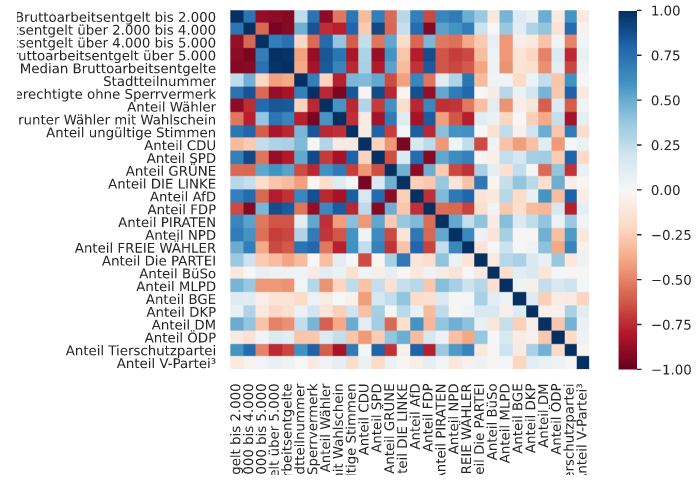
\includegraphics[width=0.8\textwidth]{figure/correlation}
	}
	\caption{Pearson-Korrelation der Daten}
	\label{fig:correlation}
\end{figure}
 stellt die Pearson-Korrelation der Daten da. Einige Zusammenhänge fallen schnell ins Auge, so hat z. B. die FDP eine sehr starke (Anti-)Korrelation zur Gehaltsgruppe 2000-bis-4000. Nicht minder stark (anti-)korreliert das Wahlergebnis der CDU mit dem der DIE LINKE. Auf jeden Fall legt die Matrix eine Korrelation zwischen Einkommen und Wahlverhalten Nahe. Weitere Untersuchungen scheinen sinnvoll. 

\subsection{Test and verify your data quality}
\TODO \emph{Ich bin mit diesem Abschnitt nicht zufrieden. Erlich gesagt, ahbe ich keine Ahnung was genau hier erwartet wird.}

Nach dem Abschluss der Analyse der Daten mit Pandas-Profiling haben wir einen Guten Überblick über die Qualität der Daten. Im Zusammenhang Mit Daten-Qualität unterschiedliche Kriterien. Wichtige sind unter andere Accuray, Relevancy, Completeness, Timliness und Consistency (\href{https://towardsdatascience.com/7-steps-to-ensure-and-sustain-data-quality-3c0040591366}{source}).
\begin{description}
\item[Accuray] Die Daten wurden von der Stadt Frankfurt erhoben und sind damit so akkurat wie möglich. Bei dem mergen der Daten, haben wir sichergestellt die Bedeutung der Daten nicht zu verändern.
\item[Relevancy] Für unsere Zwecke sind die Daten geeignet.
\item[Completness] Leider fehlen einige Informationen zu Stadtteilen. Uns bleibt nichts anderes übrig, als diese Datenpunkte für die ML-Modelle nicht zu verwenden. Uns gehen so zwei Datenpunkte verloren.
\item[Timliness] Die Daten sind die aktuellsten, die wir gefunden haben.
\item[Consitency] Unsere Daten verwenden überall die selben Datentypen. Euro für die Angaben des Einkommen und Prozentangaben für das Wahlergebnis
\end{description}


\subsection{Further preprocessing}
Die eben erwähnten Datenpunkte mit fehlenden Werten werden entfernt. Nun sind die Daten bereit, um ML-Modelle zu trainieren.


\section{Apply two different algorithms of the same kind}
Wir wollen ML-Modelle trainieren, die Vorhersagen über die Verteilung der Wahlstimmen in abhängig zu den Einkommen eines Stadtteils treffen. Trifft ein solches Modell gute Vorhersagen, würde dies unsere These unterstützen.

Die Werte die wir bestimmen wollen, sind Anteil an den Gesamtstimmen in Prozent. Das heißt wir wollen Werte von 0 bis 100 für jede Partei als Ergebnis unserer Vorhersage. Um ein solches Problem zu lösen, bietet sich Multi-Target-Regression an. scikit-learn stellt solche Funktionalität u.a. mit der Klasse \href{https://scikit-learn.org/stable/modules/generated/sklearn.multioutput.MultiOutputRegressor.html}{MultiOutputRegressor} zur Verfügung. Mit ihr ist es leicht gängige scikit-learn Regressionsmodelle für Multi-Target Probleme zu erweitern. Zwei der von uns getesteten Modelle sind \lstinline|GradientBoostingRegressor| und \lstinline|RandomForestRegressor|.
\begin{description}
	\item[GradientBoosting] baut ein additives Modell schrittweise auf. Es ermöglicht die Optimierung beliebig differenzierbarer Verlustfunktionen. In jeder Stufe wird ein Regressionsbaum an den negativen Gradienten der gegebenen Verlustfunktion angepasst
	\item[RandomForest] ist ein Meta-Schätzer, der eine Reihe von klassifizierenden Entscheidungsbäumen für verschiedene Teilstichproben des Datensatzes anpasst und mithilfe der Mittelwertbildung die Vorhersagegenauigkeit verbessert und Overfitting kontrolliert.	 
\end{description}
 Wir haben diverse Tests durchgeführt.
 \subsection{Simples Training}
 Das erste Training wurde folgendermaßen aufgebaut. Zunächst wurden die Daten in Training- und Testdaten aufgeteilt. Dazu ist die Methode \href{https://scikit-learn.org/stable/modules/generated/sklearn.model_selection.train_test_split.html}{\lstinline|train_test_split|} nützlich. Anschließend wird über die Methode \lstinline|fit| der Instanzen der Regressorklassen mit den Trainingsdaten die Modelle trainiert. Um die erzeugten Modelle auszuwerten, können wir uns die Vorhersagen der Modelle für die Testdaten anschauen. Diese erhält man durch die Methode \lstinline|predict|. Nun können wir auf diese Vorhersage übliche Metriken anwenden. Das Resultat zeigt Tabelle \ref{fig:firstresult}.\begin{figure}
 	\centering
 	\fbox{	
 		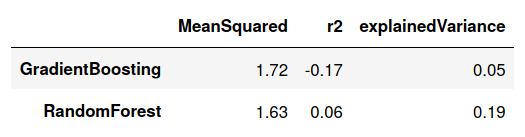
\includegraphics[width=0.6\textwidth]{figure/firstresult}
 	}
 	\caption{Metriken der ersten Modelle}
 	\label{fig:firstresult}
 \end{figure} Was bedeuten diese Werte für unsere Modelle? MeanSquared zeigt den mittleren quadratischen Fehler (MSE) über alle Datenpunkte an. Dieser Wert sag für sich selber nichts über die Güte der Modelle aus, eignet sich aber um verschiedene Modelle miteinander zu vergleichen. Ein niedrigerer Wert ist besser. Ein MSE=0 bedeutet, es gab keinerlei Fehler. Auf der Tabelle sieht man, dass RandomForest besser abgeschnitten hat als GradientBoosting.

Die bestmögliche Punktzahl, die bei $R^2$ erreicht werden kann, ist 1,0. Ein schlechteres Modell erhält einen kleineren Wert. Dieser Wert kann beliebig negativ werden. Ein konstantes Modell, das unter Berücksichtigung der Eingabemerkmale immer den erwarteten Wert von y vorhersagt, würde einen $R^2$-Wert von 0,0 erhalten. Die Werte beider Modelle sind nahe Null und Gradient Boosting sogar negativ. Sonderlich gut vorherzusagen scheinen die Modelle nicht.

Wenn $y$ der Vektor der tatsächlichen Werte ist und $\hat{y}$ die vorhergesagten Werte, dann berechnet $explained\_{}variance(y, \hat{y}) = 1 - \frac{Var\{ y - \hat{y}\}}{Var\{y\}}$ den Wert der Explained-Varianz. Der beste Wert ist 1.0, niedrigere sind schlechter. Üblicherweise sollte ein Modell einen Wert von 0.6 oder höher annehmen, um als valide zu gelten. Davon sind unsere Modelle weit entfernt.

\subsection{Erneut trainieren}
Eine mögliche Ursache für niedrige Punktzahl könnte sein, dass die Modelle im Training ein niedriges lokales Maxima erreicht haben. Um dies auszuschließen, wiederholen wir das Training auf den selben Daten $n=100$ oft. Abbildung \ref{fig:localminimum}\begin{figure}
	\centering
	\fbox{	
		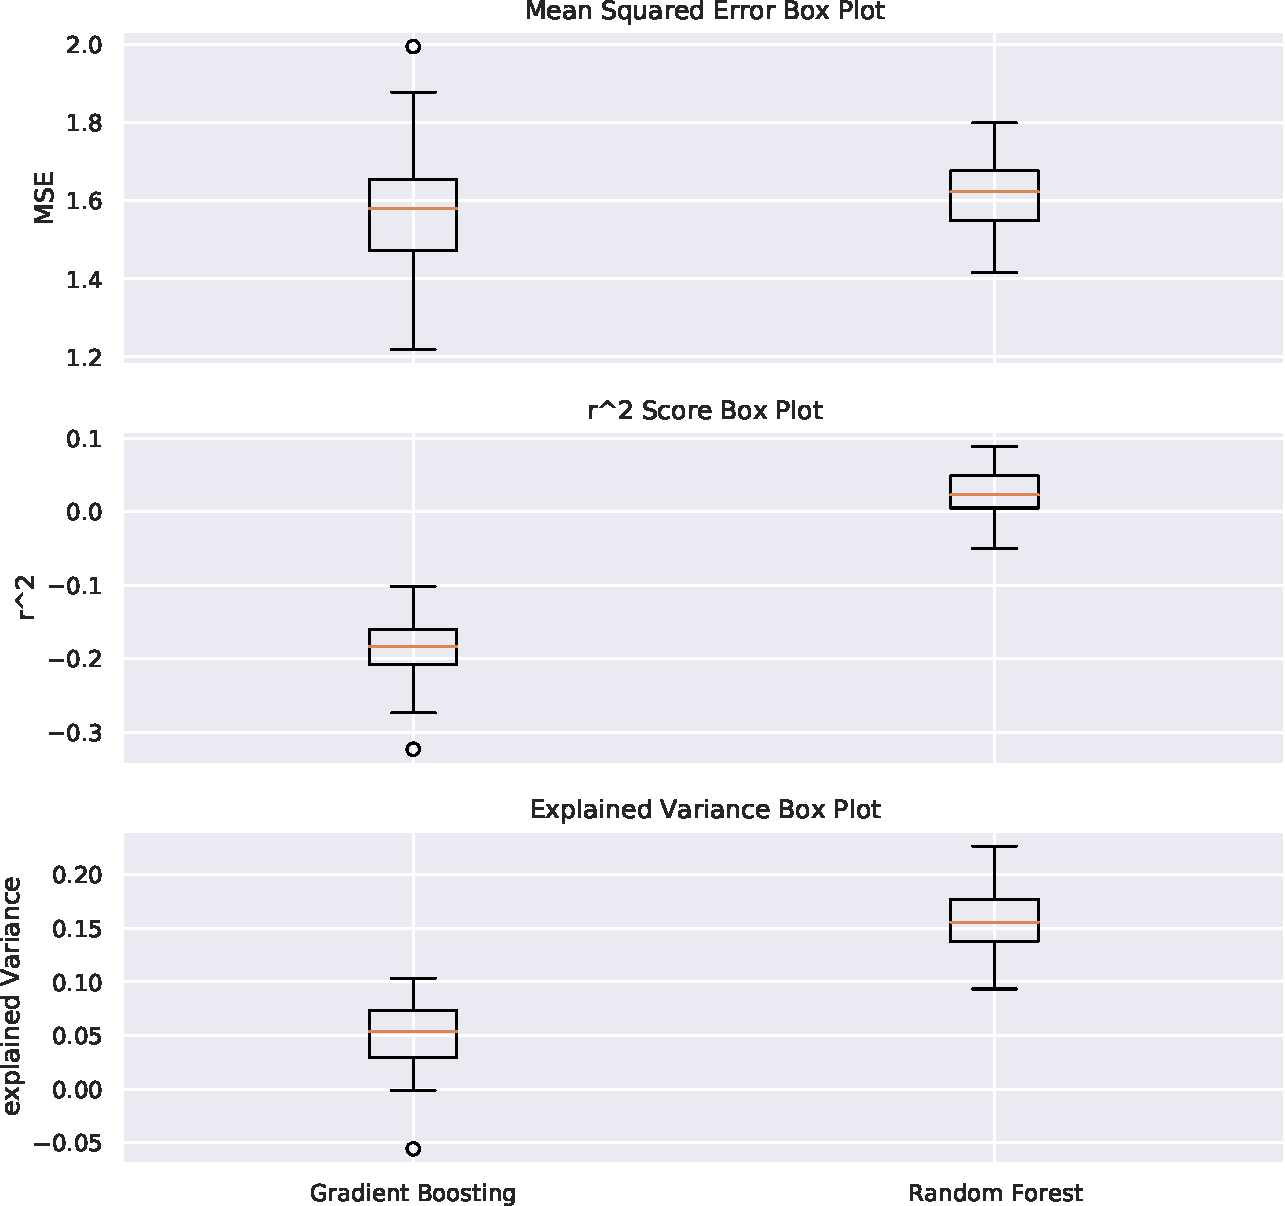
\includegraphics[width=0.6\textwidth]{figure/localminimum}
	}
	\caption{Boxplot der Metriken bei 100 Wiederholungen des Trainings auf den selben Daten}
	\label{fig:localminimum}
\end{figure} 
zeigt das Ergebnis der Auswertung. Offensichtlich spielt der Zufallsfaktor keine all zu große Rolle.
\subsection{Erneut trainieren2}
Eine weitere Quelle für ein schlechtes Ergebnis könnte ein schlechte Wahl der Trainingsdaten sein. Da unsere Menge an Daten nichts sehr groß ist, könnte dies relevant sein. Daher führen wir das Training mehrfach durch mit zufälligen Trainingsdaten und werten die Modelle aus. Die Methode, die uns diese arbeitet erleichtert ist \href{https://scikit-learn.org/stable/modules/generated/sklearn.model_selection.cross_validate.html}{\lstinline|cross\_validate|}. Das Ergebnis der Cross Validaion ist auf Abbildung \ref{fig:crossval}\begin{figure}
	\centering
	\fbox{	
		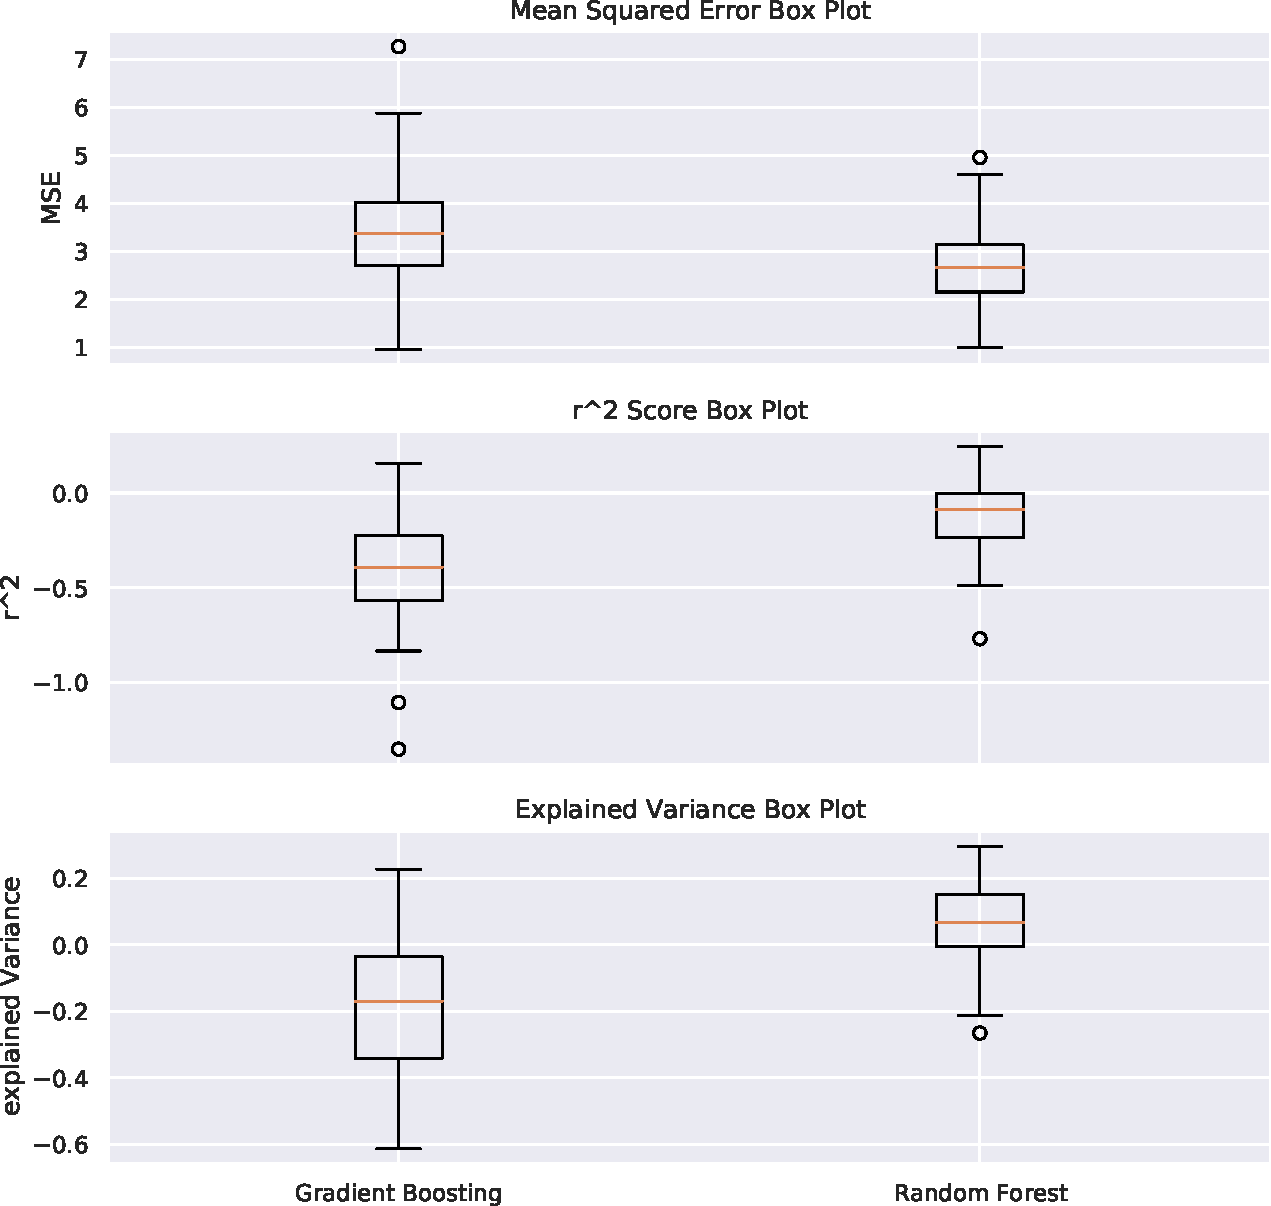
\includegraphics[width=0.6\textwidth]{figure/crossval}
	}
	\caption{Boxplot der Metriken bei 10 Wiederholungen von 5-Fold Cross Validation der Daten}
	\label{fig:crossval}
\end{figure} zu sehen. Man kann deutlich erkennen, dass die Qualität der Modelle von den gewählten Test- und Trainingsdaten abhängt. Insbesondere an der Verteilung des $R^2$-Scores kann man ablesen, dass beide Modelle in keinem Fall zu wirklich nützlich sind. Allerdings ist es noch zu früh, um aufzugeben. 
\subsection{Analyse einzelner Parteien}
Insgesamt machen die Modelle keinen guten Eindruck. Das schließt aber nicht aus, dass bei bestimmten Parteien nicht deutliche Tendenzen erkennen zu sind. Wir wiederholen die Tests und analysiere diese für einzelne Parteien. Da uns nicht jede Partei interessiert, untersuchen wir nur die großen Parteien, SPD, CDU, FDP, GRÜNE, DIE LINKE und AFD. Abbildung \ref{fig:simple_parties} \begin{figure}
	\centering
	\fbox{	
		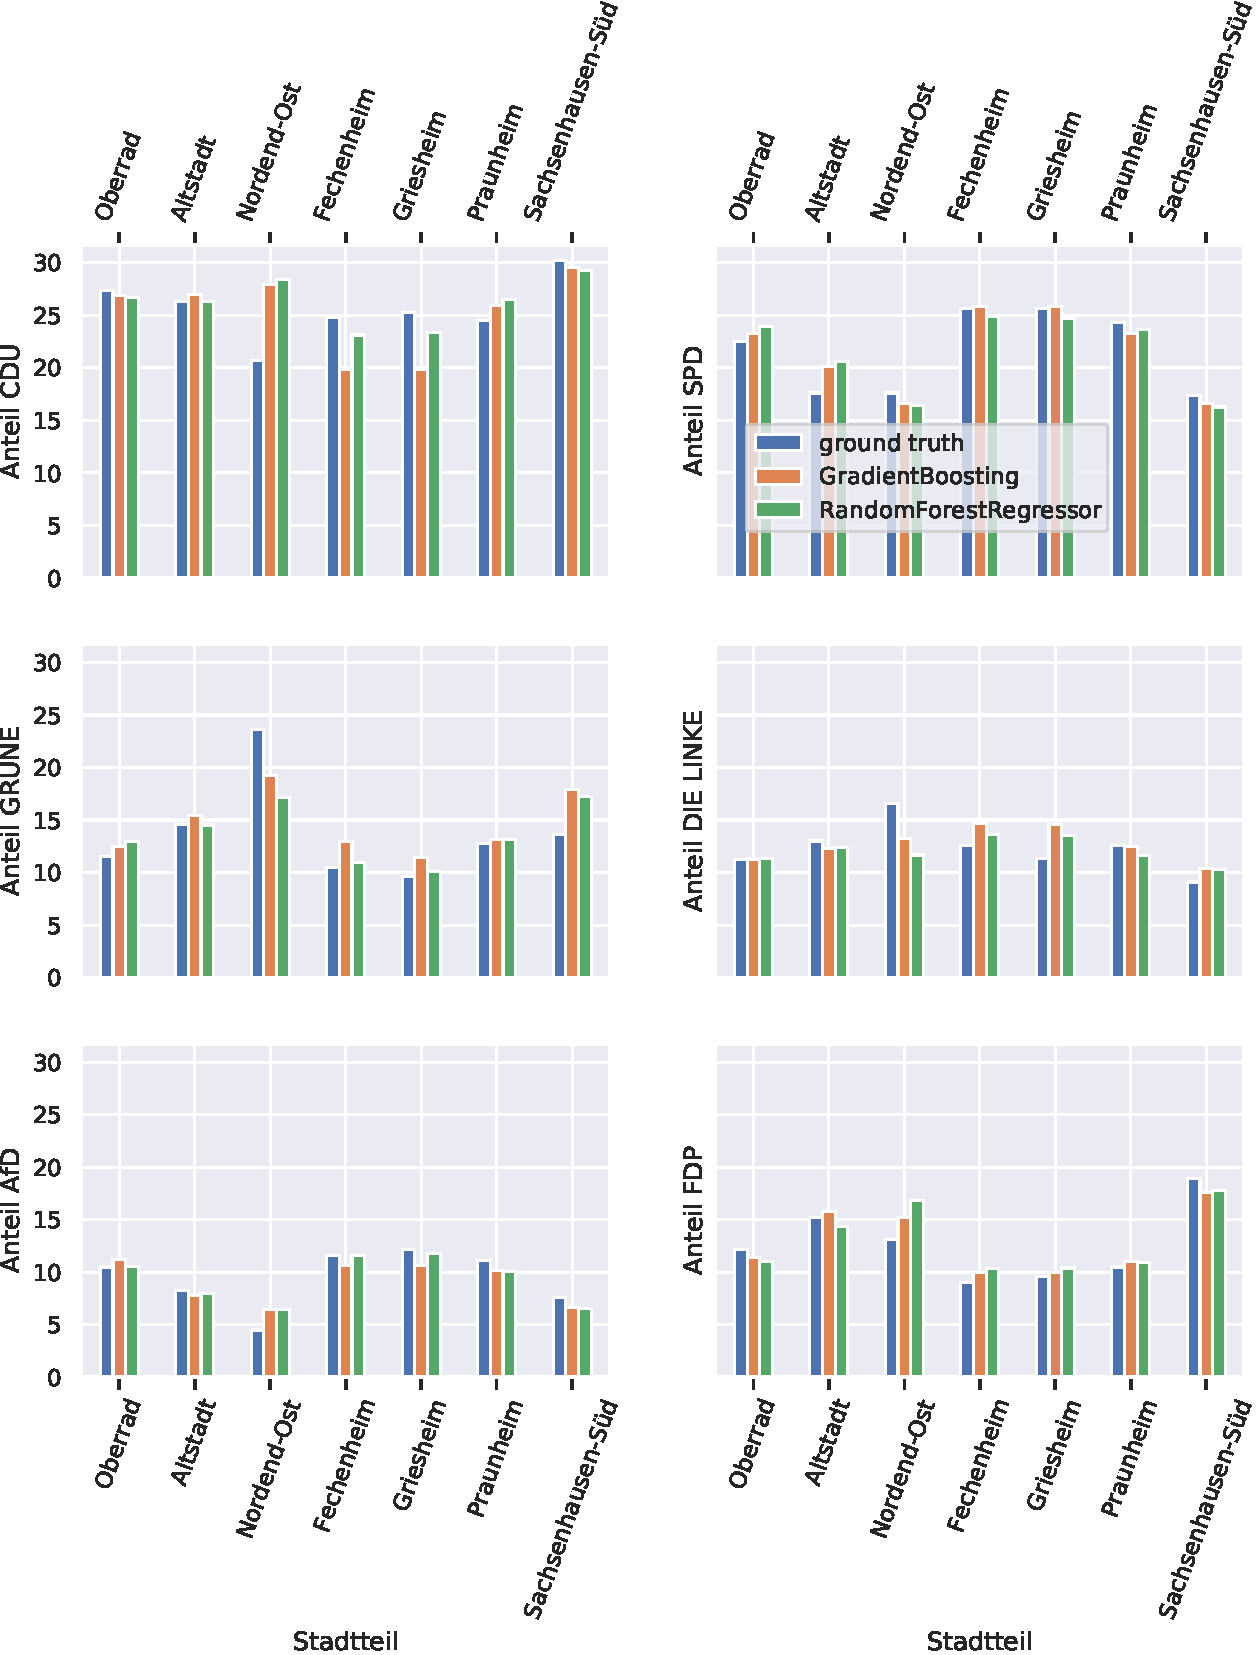
\includegraphics[width=0.9\textwidth]{figure/simple_parties}
	}
	\caption{Vergleich der Vorhersagen zweier Modelle mit der Ground Truth}
	\label{fig:simple_parties}\end{figure}  zeigt die Vorhersagen unserer beiden ersten Modelle. Man sieht, die Vorhersagen liegen nicht völlig daneben, sie sind nur oft nicht besser als ein konstantes Modell.

 Wir führen die Crossvalidation erneut durch und untersuchen diesmal die einzelnen Parteien. \ref{fig:scores_parties} \begin{figure}
 	\centering
 	\fbox{	
 		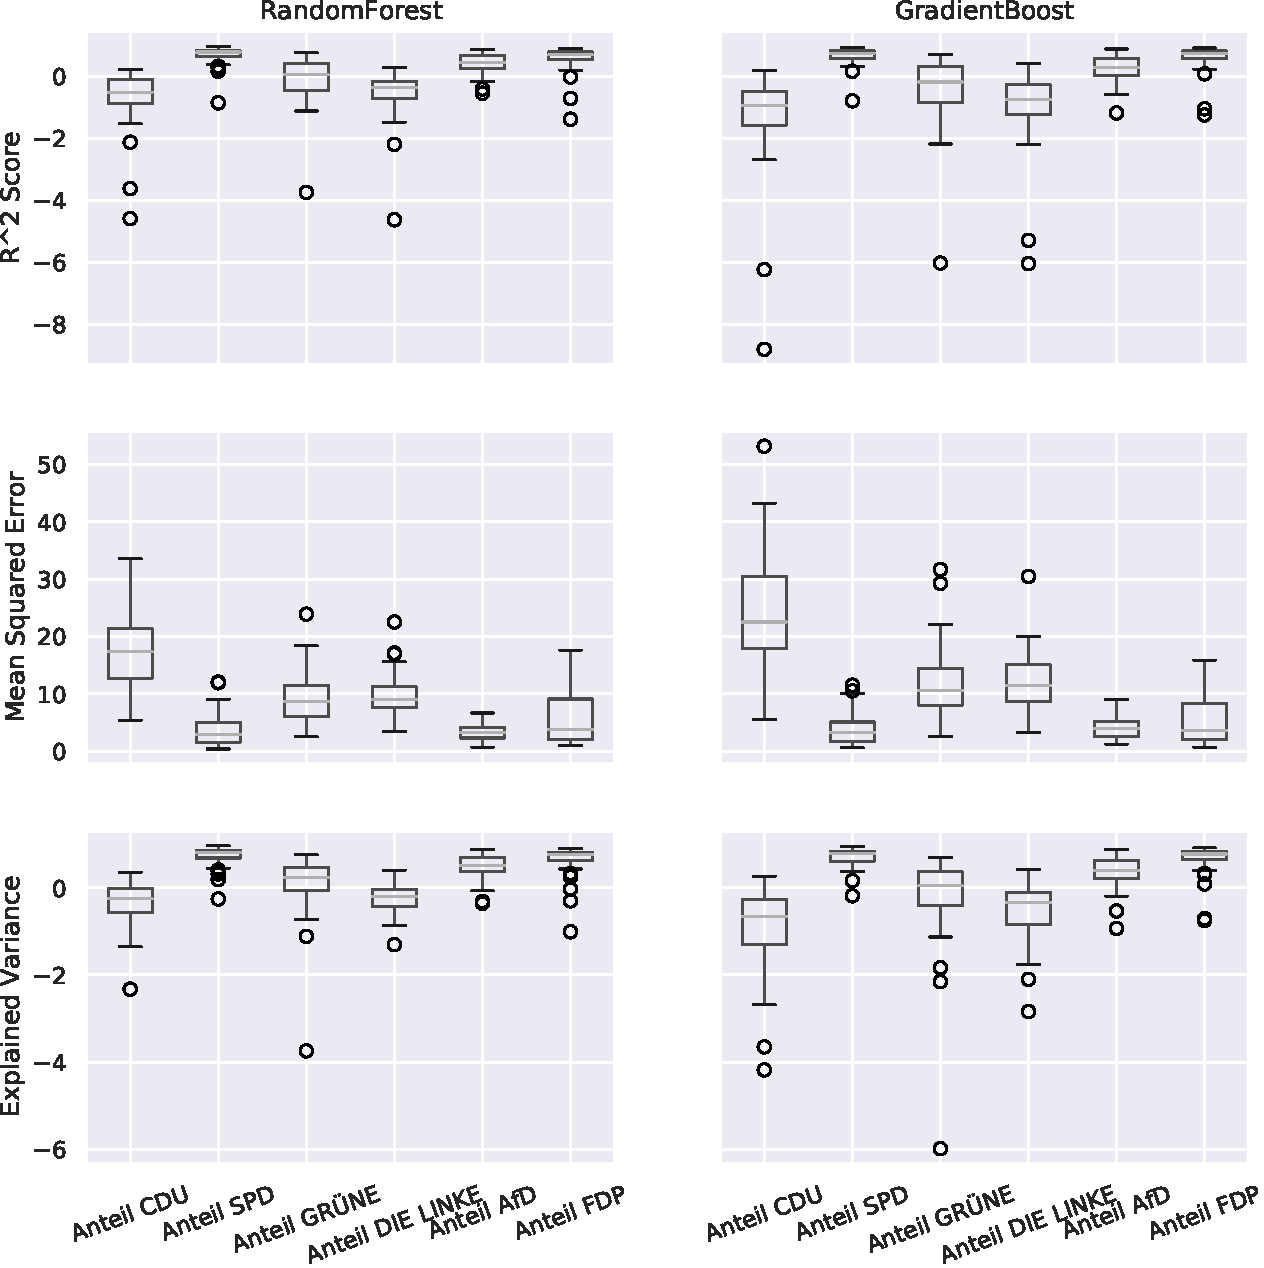
\includegraphics[width=0.9\textwidth]{figure/scores_boxplot_parties}
 	}
 	\caption{Boxplot der Punktzahl verschiedener Metriken der einzelnen Parteien}
 	\label{fig:scores_parties}\end{figure} Zum einen fällt ins Auge, dass die Varianz der Punktzahl hoch ist. Die Qualität der Modelle hängt also stark von Trainingsdaten ab. Die Menge der Trainingsdaten ist nicht ausreichend, um gute Modelle zu erstellen. Allerdings ist dies auch nicht unser Vorhaben. Wir wollen überprüfen, ob für bestimmte Parteien eine deutliche Abhängigkeit zu den Eingabedaten abzulesen ist. Tatsächlich sehen wir drei Parteien, SPD, DIE LINKE und AFD, für die im Schnitt die Modelle deutlich besser als ein vergleichbares konstantes Modell sind. Dies können wir daran ablesen, dass dort der $R^2$-Score und die Explained Varianz meist über 0 sind. Gleichzeitig ist für die Parteien der Mean Squared Error deutlich niedriger als für den Rest der Parteien. 
 


\section{Konklusion}
Die entwickelten Modelle unterstützen unsere These. Wir können deutlich sehen, dass die Modelle nützliche Vorhersagen über das Wahlverhalten treffen können. Überraschend war, dass die Modelle für bestimmte Parteien, insbesondere CDU und Grüne, sehr schlecht waren (Quelle). Wir schließen daraus, aus den Daten können keine signifikanten Schlüsse von Einkommen eines Stadtteils auf das Wahlergebnis dieser Parteien geschlossenen werden. Anders sieht es mit den Parteien DIE LINKE, SPD und AFD aus. Die Modelle können zwar nicht mit einer besonderen Zuverlässigkeit die Wahlergebnisse vorhersagen (Quelle), jedoch sind die Ergebnisse so gut, dass wir klar sagen können, die Einkommensverteilung eines Stadtteils hat Einfluss auf das Wahlergebnis. Ohne weitere Untersuchung können wir allerdings nicht sagen, welche Art von Einkommensverteilung eine bestimmte Partei bevorzugt. 
\end{document}
